\documentclass[12pt]{article}
\usepackage{amsmath, amssymb}
\usepackage{geometry}
\usepackage{listings}
\usepackage{xcolor}
\usepackage{booktabs}
\usepackage{parskip}
\usepackage{hyperref}
\usepackage{graphicx}

\geometry{margin=1in}

\definecolor{codebg}{rgb}{0.95,0.95,0.95}
\definecolor{codegreen}{rgb}{0,0.5,0}
\definecolor{codepurple}{rgb}{0.5,0,0.5}
\definecolor{codeblue}{rgb}{0,0,0.7}

\lstset{
    backgroundcolor=\color{codebg},
    basicstyle=\ttfamily\small,
    keywordstyle=\color{codeblue}\bfseries,
    commentstyle=\color{codegreen},
    stringstyle=\color{codepurple},
    breaklines=true,
    frame=single,
    language=Python,
    numbers=left,
    numberstyle=\tiny\color{gray},
    showstringspaces=false,
}

\title{ODE Project Phase 2}
\author{
Greyson Knippel \\[4pt]
MATH 260-1 --- Gonzaga University \\[4pt]
Professor Jensen
}
\date{\today}

\begin{document}
\maketitle

% -------------------------------------------------------
\section{part 1: F = ma}
% -------------------------------------------------------

\begin{itemize}
    \item \textbf{gravity:} $F_g = -mg$ \quad (downward, hence negative)
    \item \textbf{linear spring:} $F_k = -kx$
    \item \textbf{nonlinear spring:} $F_a = -ax^3$
    \item \textbf{shock damper:} $F_b = -b\dot{x}$
\end{itemize}


summing all forces on the probe:
\[
    m\ddot{x} = -mg - kx - ax^3 - b\dot{x}
\]

rearranging by moving all terms to the left side:
\[
    \boxed{m\ddot{x} + b\dot{x} + kx + ax^3 = -mg}
\]


when the probe is compressed downward, $x < 0$. the spring forces become:
\[
    -kx = -k(\text{negative}) > 0 \quad \text{(upward)} \checkmark
\]
\[
    -ax^3 = -a(\text{negative})^3 > 0 \quad \text{(upward)} \checkmark
\]


% -------------------------------------------------------
\section{part 2: spring limit}
% -------------------------------------------------------
when the probe rests at rest on the surface, $\dot{x} = 0$ and $\ddot{x} = 0$.
\[
    kx + ax^3 = -mg
\]


\begin{align*}
    m &= 1{,}220 \text{ kg} \\
    k &= 35{,}600 \text{ N/m} \\
    g &= 17.5 \text{ m/s}^2 \\
    mg &= 1{,}220 \times 17.5 = 21{,}350 \text{ N}
\end{align*}

the equilibrium eq is:
\[
    35{,}600\, x + a\, x^3 = -21{,}350
\]

we require the compression $|x|$ to be as close to $0.3$ m as possible \textit{without exceeding} $0.3$ 

\subsection{$x = -0.3$ m}

substituting $x = -0.3$ m, the spring force is:
\[
    35{,}600(0.3) + a(0.3)^3 = 10{,}680 + 0.027a
\]

comparing to the required $mg = 21{,}350$ N:

\begin{center}
\begin{tabular}{cccc}
\toprule
$a$ (N/m$^3$) & force at $x=-0.3$ (N) & vs.\ $mg$ & compression \\
\midrule
150,000 & 14,730 & too small & exceeds 0.3 m $\times$ \\
300,000 & 18,780 & too small & exceeds 0.3 m $\times$ \\
450,000 & 22,830 & good & under 0.3 m $\checkmark$ \\
600,000 & 26,880 & good & under 0.3 m $\checkmark$ \\
\bottomrule
\end{tabular}
\end{center}


only $a = 450{,}000$ and $a = 600{,}000$ N/m$^3$ satisfy the 0.3 value. between these, $a = 450{,}000$ N/m$^3$ gives the greatest fit. solving this gives a compression of  $x \approx -0.287$ m.

% -------------------------------------------------------
\section{part 3: damping coeff.}
% -------------------------------------------------------

to use the numerical ODE solver, the second-order equation is rewritten as a system of two first-order equations. Let $x_1 = x$ and $x_2 = \dot{x}$:

\begin{align*}
    \dot{x}_1 &= x_2 \\
    \dot{x}_2 &= \frac{1}{m}\left(-mg - bx_2 - kx_1 - ax_1^3\right)
\end{align*}

\subsection{initial conditions}

at moment of impact:
\begin{align*}
    x(0) &= 0 \quad \text{(springs at natural length)} \\
    \dot{x}(0) &= -V_L = -5 \text{ m/s} \quad \text{(downward = negative)}
\end{align*}

\subsection{python code for ODE solver}

\begin{lstlisting}[caption={numerical integration to find minimum $b$}]
import numpy as np
from scipy.integrate import solve_ivp
import matplotlib.pyplot as plt

# parameters/given stuff
m = 1220        # kg
k = 35600       # N/m
g = 17.5        # m/s^2
a = 450000      # N/m^3 (from question 2)
VL = 5.0        # m/s (impact velocity)

# ODE system: state = [x, x_dot]
def landing_ode(t, y, b):
    x, x_dot = y
    x_ddot = (-m*g - b*x_dot - k*x - a*x**3) / m
    return [x_dot, x_ddot]

# initial conditions
y0 = [0, -VL]

# time span
t_span = (0, 20)
t_eval = np.linspace(0, 20, 10000)

# test each b value
b_values = np.arange(1000, 10500, 500)
results = {}

for b in b_values: #for each b inthe values array we made earlier
    sol = solve_ivp(landing_ode, t_span, y0, args=(b,),
                    t_eval=t_eval, max_step=0.001)
    max_x = np.max(sol.y[0])
    results[b] = max_x
    status = "OK" if max_x <= 0 else "REBOUND"
    print(f"b = {b:6.0f} N*s/m | max x = {max_x:.6f} m | {status}")

# find minimum valid b
valid_b = [b for b, max_x in results.items() if max_x <= 0]
b_min = min(valid_b)
print(f"\nMinimum valid b = {b_min} N*s/m")

# plot result for minimum b with matplotlib
sol = solve_ivp(landing_ode, t_span, y0, args=(b_min,),
                t_eval=t_eval, max_step=0.001)

plt.figure(figsize=(10, 5))
plt.plot(sol.t, sol.y[0], label=f'b = {b_min} N*s/m')
plt.axhline(0, color='red', linestyle='--', label='x = 0 (natural length)')
plt.xlabel('Time (s)')
plt.ylabel('Displacement x (m)')
plt.title('Probe Displacement After Impact')
plt.legend()
plt.grid(True)
plt.savefig('displacement.png', dpi=150, bbox_inches='tight')
plt.show()
\end{lstlisting}

\begin{figure}[h]
    \centering
    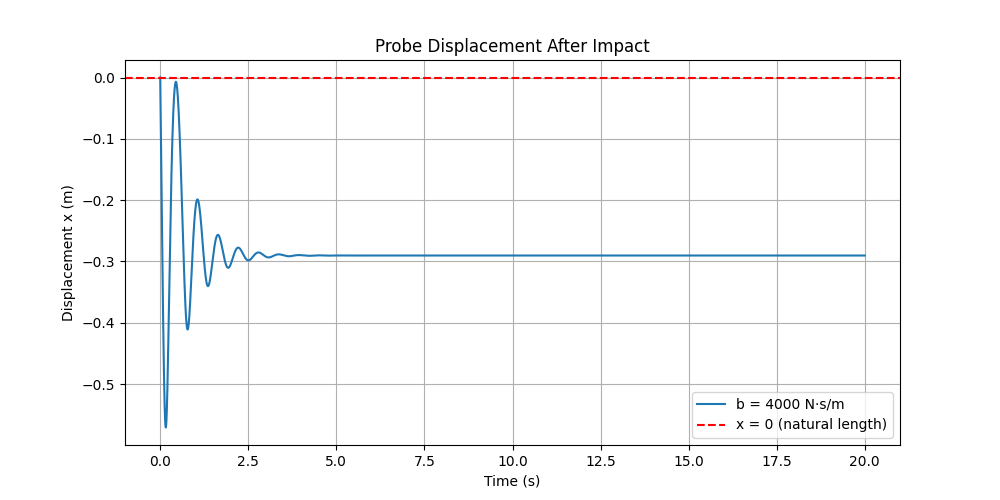
\includegraphics[width=\textwidth]{phase2fig1.png}
    \caption{probe displacement after impact for minimum $b$}
    \label{fig:displacement}
\end{figure}

\end{document}